\chapter{Photochemistry}\label{ch:b3:photochemistry}

Vision begins when one photon bends one molecule. In the rod cells of the eye,
retinal sits in its protein in the 11-cis form; a photon of green light turns
it into the all-trans form, and the isomerisation is essentially complete
within \qty{200}{fs}, faster than almost any other chemical event. The rest of
vision, an enormous biochemical amplification, follows from that single bent
molecule. The same rules (one photon excites one molecule, which then chooses
among several fates) govern sunscreens, the synthesis of strained rings,
photodynamic therapy, the smog over cities and the \omterm{def:b3:photochemistry:chapman}{ozone layer} that shields
the surface of the Earth from ultraviolet light.

\begin{recall}
\Cref{ch:b3:electronic-spectroscopy} described the excited states of
molecules, the \omterm{def:b3:electronic-spectroscopy:jablonski}{Jablonski diagram}, \omterm{def:b3:electronic-spectroscopy:radiationless}{intersystem crossing}, \omterm{def:b3:electronic-spectroscopy:luminescence}{fluorescence} and
\omterm{def:b3:electronic-spectroscopy:luminescence}{phosphorescence}, quenching and the \omterm{def:b3:electronic-spectroscopy:quantum-yield}{quantum yield} of a photophysical process.
The Year 1 volume defined radicals, homolysis and $Z$/$E$ isomers; the Year 2
volume concerted reactions, frontier orbitals and catalytic cycles.
\Cref{ch:b3:complex-kinetics} treated \omterm{def:b3:complex-kinetics:chain}{chain reactions} and steady states.
\end{recall}

\section{Light as a reagent}

Two old principles start the subject: only light that is absorbed can cause a
chemical change (Grotthuss and Draper), and each absorbed photon excites one
molecule (Stark and Einstein).

\begin{definition}[Photon flux, chemical actinometer]\label{def:b3:photochemistry:photon-flux}
The \emph{photon flux}\index{photon flux} of a light source is the number of
photons it delivers per unit time, often counted in moles of photons (einstein)
per second. A \emph{chemical actinometer}\index{chemical actinometer} is a
photochemical reaction of accurately known \omterm{def:b3:electronic-spectroscopy:quantum-yield}{quantum yield} used to measure a
photon flux.
\end{definition}

\begin{proposition}[Stark--Einstein law]\label{prop:b3:photochemistry:stark-einstein}
In ordinary light intensities, each absorbed photon excites exactly one
molecule; the primary \omterm{def:b3:electronic-spectroscopy:quantum-yield}{quantum yields} of all the processes that start from the
excited state add up to 1.
\end{proposition}

\begin{proof}[Partial proof]
That one photon is absorbed by one molecule at a time is admitted (two-photon
absorption needs the intensities of pulsed lasers). The excited molecule then
disappears by competing first-order processes of rate constants $k_i$
(\cref{ch:b3:electronic-spectroscopy}): the fraction that takes path $i$ is $\Phi_i =
k_i/\sum_jk_j$, and $\sum_i\Phi_i = 1$.
\end{proof}

The \omterm{def:b3:electronic-spectroscopy:quantum-yield}{quantum yield} of a reaction, the number of molecules converted per photon
absorbed, need not obey this limit: a primary photochemical step can start a
chain. A mixture of \ce{H2} and \ce{Cl2} exposed to light reacts with \omterm{def:b3:electronic-spectroscopy:quantum-yield}{quantum yields}
of $10^4$ and more, each photolysed \ce{Cl2} starting a chain like that of the
hydrogen--bromine reaction of \cref{ch:b3:complex-kinetics}; a \omterm{def:b3:electronic-spectroscopy:quantum-yield}{quantum yield}
larger than 1 is the signature of a chain.

\begin{proposition}[Rate of a photochemical reaction]\label{prop:b3:photochemistry:rate}
A solution of absorbance $A$ at the irradiation wavelength, receiving a \omterm{def:b3:photochemistry:photon-flux}{photon
flux} $I_0$ (einstein per second), absorbs $I_{\mathrm{abs}} = I_0(1 - 10^{-A})$; if the
reactant absorbs all of it, the reaction converts $v = \Phi I_{\mathrm{abs}}$ moles per second.
\end{proposition}

\begin{proof}
By the Beer--Lambert law the transmitted flux is $I_010^{-A}$, so the absorbed one
is $I_0(1 - 10^{-A})$; by definition of the \omterm{def:b3:electronic-spectroscopy:quantum-yield}{quantum yield}, $\Phi$ molecules react per
photon absorbed.
\end{proof}

\begin{method}[The rate of a photoreaction from the lamp]\label{met:b3:photochemistry:photochemical-rate}
\begin{enumerate}
  \item Photon energy $E = hc/\lambda$; \omterm{def:b3:photochemistry:photon-flux}{photon flux} $I_0 = P/E$ for a power $P$ reaching the
        sample, or measured with an actinometer; divide by $N_A$ for einstein per
        second.
  \item Absorbed fraction $1 - 10^{-A}$, with $A$ at the irradiation wavelength (it
        changes as the reactant is consumed).
  \item Rate $\Phi I_{\mathrm{abs}}$ in mol/s, divided by the volume for a concentration rate.
\end{enumerate}
\end{method}

\begin{method}[Ferrioxalate actinometry]\label{met:b3:photochemistry:actinometry}
\begin{enumerate}
  \item Irradiate, in the same cell and geometry as the experiment, an acidified
        solution of potassium tris(oxalato)ferrate(III), concentrated enough to
        absorb practically all the light below about \qty{450}{nm}.
  \item Light reduces Fe(III) to Fe(II) with a calibrated \omterm{def:b3:electronic-spectroscopy:quantum-yield}{quantum yield}; after a
        measured time, add 1,10-phenanthroline and buffer, and measure the
        absorbance of the red $\ce{[Fe(phen)3]^{2+}}$ complex.
  \item Moles of Fe(II) divided by (\omterm{def:b3:electronic-spectroscopy:quantum-yield}{quantum yield} $\times$ time) give the \omterm{def:b3:photochemistry:photon-flux}{photon flux}.
\end{enumerate}
\end{method}

\section{Photochemical reactions}

\begin{definition}[Photoisomerisation, photostationary state]\label{def:b3:photochemistry:photoisomerisation}
A \emph{photoisomerisation}\index{photoisomerisation} is a light-induced
conversion of one isomer into another, typically $E \to Z$ about a double bond. Under
continuous irradiation two isomers that both absorb reach a
\emph{photostationary state}\index{photostationary state}, a steady composition
set by the light, not by thermodynamics.
\end{definition}

The twisting of a double bond explains why light isomerises alkenes. In the
ground state the energy rises as the two ends twist, to a maximum at $90^\circ$
where the $\pi$ bond is broken. In the $\pi\pi^*$ excited state the order is reversed: the
twisted geometry is the most stable. An excited molecule twists towards
$90^\circ$, where the two surfaces come together, crosses back to the ground state
there, and falls to either side: to the isomer it started from or to the other
one.

\begin{omfigure}
\begin{tikzpicture}[font=\small, >=Stealth, x=0.032cm, y=1.1cm]
  \draw[->] (0,0) -- (195,0);
  \node[anchor=north] at (135,-0.45) {twist angle};
  \draw[->] (0,0) -- (0,5.2) node[anchor=south] {energy};
  \foreach \t/\l in {0/{0^\circ}, 90/{90^\circ}, 180/{180^\circ}}{
    \draw (\t,0) -- (\t,-0.08) node[anchor=north] {$\l$};}
  \draw[thick, black, domain=0:180, samples=90] plot (\x,{2.6*sin(\x)^2 + 0.15*(1-cos(\x))/2});
  \draw[thick, omThm, domain=0:180, samples=90] plot (\x,{4.5 - 1.6*sin(\x)^2 + 0.1*(1-cos(\x))/2});
  \node[anchor=east] at (0,0.15) {$E$};
  \node[anchor=west] at (182,0.2) {$Z$};
  \node[omThm, anchor=south west] at (5,4.55) {$\mathrm S_1$ ($\pi\pi^*$)};
  \node[anchor=north west] at (52,1.2) {$\mathrm S_0$};
  \draw[->, omDef, thick] (12,0.12) -- (12,4.4) node[midway, left] {$h\nu$};
  \draw[->, omDef, thick, decorate, decoration={snake, amplitude=0.6mm, segment length=3mm}] (16,4.4) -- (80,3.05);
  \draw[->, omDef, thick] (90,2.85) -- (90,2.75);
  \draw[->, black!60, thick, domain=96:168, samples=40] plot (\x,{2.6*sin(\x)^2 + 0.15*(1-cos(\x))/2 + 0.28});
  \draw[->, black!60, thick, domain=84:12, samples=40] plot (\x,{2.6*sin(\x)^2 + 0.15*(1-cos(\x))/2 + 0.28});
  \node[font=\scriptsize, anchor=south, align=center] at (90,3.05) {funnel};
\end{tikzpicture}

{\small Ground state ($\mathrm S_0$) and first excited state ($\mathrm S_1$) of an alkene against the
twist of its double bond (schematic). Excitation of the $E$ isomer (vertical arrow)
is followed by twisting on $\mathrm S_1$ to the perpendicular geometry, where the two
surfaces nearly touch; the molecule returns to $\mathrm S_0$ there and relaxes to $E$ or to
$Z$.}
\end{omfigure}

\begin{proposition}[Photostationary composition]\label{prop:b3:photochemistry:pss}
Under monochromatic irradiation of an optically thin solution, two isomers $E$
and $Z$ with absorption coefficients $\varepsilon_E$, $\varepsilon_Z$ and \omterm{def:b3:electronic-spectroscopy:quantum-yield}{quantum yields} $\Phi_{E\to Z}$,
$\Phi_{Z\to E}$ reach the photostationary ratio
\[
  \frac{[Z]}{[E]} = \frac{\varepsilon_E\Phi_{E\to Z}}{\varepsilon_Z\Phi_{Z\to E}} .
\]
\end{proposition}

\begin{proof}
In an optically thin sample each isomer absorbs a flux proportional to $\varepsilon[\cdot]$, so
$\dd[Z]/\dd t = c(\varepsilon_E\Phi_{E\to Z}[E] - \varepsilon_Z\Phi_{Z\to E}[Z])$ with a constant $c$ fixed by the light;
the steady state sets the bracket to zero. (The result holds also for thick
samples, both isomers then sharing the absorbed light in the same proportion.)
\end{proof}

\begin{omfigure}
\begin{tikzpicture}
\begin{axis}[width=0.7\linewidth, height=5.0cm, xmin=0, xmax=120, ymin=0, ymax=1,
  axis lines=left, xlabel={irradiation time / s}, ylabel={fraction of $Z$},
  tick label style={font=\small}, label style={font=\small}]
\addplot[omDef, very thick] table[x=t, y=Z] {figdata/out/bachelor-3-photostationary.dat};
\draw[black!35, densely dotted] (axis cs:0,0.801) -- (axis cs:60,0.801);
\draw[black!35, densely dotted] (axis cs:60,0.161) -- (axis cs:120,0.161);
\draw[black!35] (axis cs:60,0) -- (axis cs:60,1);
\node[font=\scriptsize, anchor=north] at (axis cs:30,0.98) {\qty{365}{nm}};
\node[font=\scriptsize, anchor=north] at (axis cs:90,0.98) {\qty{440}{nm}};
\node[font=\scriptsize, anchor=south east] at (axis cs:58,0.81) {pss 0.80};
\node[font=\scriptsize, anchor=south east] at (axis cs:118,0.17) {pss 0.16};
\end{axis}
\end{tikzpicture}

{\small A model photoswitch (an azobenzene-like molecule) irradiated at \qty{365}{nm}, where
the $E$ isomer absorbs much more strongly, then at \qty{440}{nm}, where the $Z$ isomer does:
the composition switches between two \omterm{def:b3:photochemistry:photoisomerisation}{photostationary states} (model
absorption coefficients and \omterm{def:b3:electronic-spectroscopy:quantum-yield}{quantum yields}).}
\end{omfigure}

The 11-cis to all-trans isomerisation of retinal in rhodopsin is such a
reaction, made exceptionally fast and selective by the protein. Synthetic
photoswitches built on azobenzene or stilbene are used to control molecular
machines, materials and, attached to drugs or ion channels, biological
activity with light.

\begin{definition}[Photolysis]\label{def:b3:photochemistry:photolysis}
\emph{Photolysis}\index{photolysis} is the breaking of a bond by light. In the
atmosphere, the first-order rate constant $j$ of the photolysis of a species, its
\emph{photolysis rate constant}\index{photolysis rate constant}, sums over
wavelengths the solar \omterm{def:b3:photochemistry:photon-flux}{photon flux} times the absorption cross-section times the
\omterm{def:b3:electronic-spectroscopy:quantum-yield}{quantum yield}.
\end{definition}

A photon breaks a bond only if its energy exceeds the dissociation energy:
$\lambda < hcN_A/D_0$. For \ce{O2}, $D_0 = 2\Delta_fH^\circ_0(\ce{O}) = \qty{493.6}{kJ/mol}$ from the thermochemical
tables, and only light shorter than \qty{242}{nm} can split it.

Excited ketones and alkenes also form bonds. Two alkenes, one of them excited,
combine into a cyclobutane: the $[2+2]$ photocycloaddition, forbidden in the
ground state and allowed in the excited state for orbital reasons given in
\cref{ch:b3:pericyclic}. It makes four-membered rings, strained and otherwise
hard to reach, in one step.

\begin{definition}[Norrish reactions]\label{def:b3:photochemistry:norrish}
A \emph{Norrish type I reaction}\index{Norrish type I reaction} is the cleavage, by
an excited ketone, of the bond between the carbonyl carbon and an $\alpha$ carbon,
into an acyl and an alkyl radical. A \emph{Norrish type II
reaction}\index{Norrish type II reaction} is the abstraction, by the oxygen of an
excited ketone, of a hydrogen atom from the $\gamma$ carbon, giving a 1,4-biradical
that either cleaves into an enol and an alkene or closes into a cyclobutanol.
\end{definition}

\begin{omfigure}
\setchemfig{atom sep=1.9em}
\schemestart
\chemfig{H_3C-[:30]C(=[:90]O)-[:-30]CH_2-[:30]CH_2-[:-30]CH_2-[:30]CH_3}
\arrow{->[$h\nu$][via $\mathrm T_1$]}
\chemfig{H_3C-[:30]\chembelow{C}{\scriptstyle\bullet}(-[:90]OH)-[:-30]CH_2-[:30]CH_2-[:-30]\chemabove{C}{\scriptstyle\bullet}H-[:30]CH_3}
\schemestop

\medskip
\schemestart
\arrow{->[cleavage]}[,1.1]
\chemfig{H_3C-[:30]C(-[:90]OH)=[:-30]CH_2}
\+
\chemfig{H_2C=[:30]CH-[:-30]CH_3}
\schemestop
\hspace{2.5em}
\schemestart
\arrow{->[ring][closure]}[,1.1]
\chemfig{*4(-(-[::-40]OH)(-[::40]CH_3)-(-CH_3)---)}
\schemestop
\par\medskip

{\small The \omterm{def:b3:photochemistry:norrish}{Norrish type II reaction} of hexan-2-one. The triplet ketone abstracts
a hydrogen from the $\gamma$ carbon through a six-membered arrangement; the 1,4-biradical
cleaves into the enol of acetone (which tautomerises to acetone) and propene,
or closes into 1,2-dimethylcyclobutan-1-ol.}
\end{omfigure}

The photoreduction of benzophenone is the classic bimolecular version: its
triplet abstracts a hydrogen atom from an alcohol solvent such as propan-2-ol,
and two of the resulting diphenylhydroxymethyl radicals couple into benzopinacol,
which crystallises from the solution.

\section{Photosensitisation}

\begin{definition}[Photosensitisation, singlet oxygen]\label{def:b3:photochemistry:sensitisation}
A \emph{photosensitiser}\index{photosensitiser} is a molecule that absorbs light
and transfers the energy or an electron to another molecule, which does not
itself absorb: this is \emph{photosensitisation}\index{photosensitisation}. In
\emph{triplet energy transfer}\index{triplet energy transfer} the \omterm{def:b3:many-electron-atoms:singlet-triplet}{triplet state} of
the sensitiser, formed by \omterm{def:b3:electronic-spectroscopy:radiationless}{intersystem crossing}, gives its energy to the
acceptor on contact, leaving the acceptor in its \omterm{def:b3:many-electron-atoms:singlet-triplet}{triplet state}. \emph{Singlet
oxygen}\index{singlet oxygen} is the lowest excited state of \ce{O2},
${}^1\Delta_g$, formed this way from ground-state ${}^3\Sigma_g^-$ oxygen.
\end{definition}

\begin{proposition}[Energy condition for triplet transfer]\label{prop:b3:photochemistry:sensitisation-condition}
Triplet--triplet energy transfer from a donor D to an acceptor A is close to the
diffusion limit when $E_{\mathrm T}(\mathrm D)$ exceeds $E_{\mathrm T}(\mathrm A)$ by more than about \qty{10}{kJ/mol}, and
falls steeply as the difference becomes negative.
\end{proposition}

\begin{proof}[Partial proof]
The transfer ${}^3\mathrm D + \mathrm A \to \mathrm D + {}^3\mathrm A$ conserves spin (two triplets exchanged for a
singlet and a triplet) and needs orbital contact (an exchange mechanism,
admitted). Its equilibrium constant is $\exp[(E_{\mathrm T}(\mathrm D) - E_{\mathrm T}(\mathrm A))/RT]$, about 60 for a
\qty{10}{kJ/mol} excess at \qty{298}{K}: the forward step then happens at nearly every
encounter. When the difference is negative, the forward rate constant is the
diffusion limit times the inverse of that factor (the uphill direction pays
the Boltzmann factor); the quantitative curve is admitted.
\end{proof}

A good sensitiser absorbs where the acceptor does not, crosses to its triplet
with a high yield, and has a long triplet lifetime: benzophenone, with a
triplet yield close to 1, is the standard. \omterm{def:b3:photochemistry:sensitisation}{Singlet oxygen} is a reactive
electrophile: it adds to dienes and to electron-rich alkenes. In photodynamic
therapy a sensitiser that accumulates in a tumour, illuminated through an
optical fibre, makes \omterm{def:b3:photochemistry:sensitisation}{singlet oxygen} that destroys the cells around it.

\begin{definition}[Photoredox catalysis]\label{def:b3:photochemistry:photoredox}
\emph{Photoredox catalysis}\index{photoredox catalysis} uses a \omterm{def:b3:photochemistry:sensitisation}{photosensitiser}
whose excited state is both a stronger oxidant and a stronger reductant than its
ground state to transfer single electrons to or from substrates, generating
radicals under visible light; the sensitiser is regenerated in a catalytic
cycle.
\end{definition}

The ruthenium complex $\ce{[Ru(bpy)3]^{2+}}$ is the prototype: its metal-to-ligand charge
transfer excited state, reached with blue light and living about a
microsecond, can take an electron from an amine or give one to an organic
halide. The radicals formed take part in bond-forming reactions under
conditions far milder than those of classical radical chemistry.

\section{Photochemistry of the atmosphere}

\begin{definition}[Chapman mechanism, ozone layer]\label{def:b3:photochemistry:chapman}
The \emph{Chapman mechanism}\index{Chapman mechanism} is the set of four steps
\[
  \ce{O2 ->[h\nu] 2 O}\ (j_1), \quad \mathrm{O + O_2 + M \to O_3 + M}\ (k_2), \quad
  \ce{O3 ->[h\nu] O2 + O}\ (j_3), \quad \ce{O + O3 -> 2 O2}\ (k_4).
\]
The \emph{ozone layer}\index{ozone layer} is the region of the stratosphere, about
15 to \qty{35}{km} above the ground, where these reactions maintain the largest
concentrations of ozone.
\end{definition}

\begin{theorem}[Chapman steady state]\label{thm:b3:photochemistry:chapman}
In the \omterm{def:b3:photochemistry:chapman}{Chapman mechanism}, O and \ce{O3} reach the steady state
\[
  \frac{[\ce{O}]}{[\ce{O3}]} = \frac{j_3}{k_2[\mathrm M][\ce{O2}]}, \qquad
  [\ce{O3}] = [\ce{O2}]\sqrt{\frac{j_1k_2[\mathrm M]}{j_3k_4}} .
\]
\end{theorem}

\begin{proof}
O and \ce{O3} interconvert quickly through steps 2 and 3 (seconds), much faster
than they are made or destroyed: setting the fast exchange to equilibrium,
$k_2[\ce{O}][\ce{O2}][\mathrm M] = j_3[\ce{O3}]$, gives the ratio. Their sum, the odd oxygen, is made by
step 1 (two O per \ce{O2}) and destroyed by step 4 (two odd oxygens per event):
$2j_1[\ce{O2}] = 2k_4[\ce{O}][\ce{O3}]$. Substituting $[\ce{O}]$ from the ratio gives $[\ce{O3}]^2 = j_1k_2[\mathrm M][\ce{O2}]^2/(j_3k_4)$.
\end{proof}

With the rate constants of the evaluated database and \omterm{def:b3:photochemistry:photolysis}{photolysis} rates typical
of \qty{30}{km} (data of the weekend problem), the Chapman model gives about
$\num{6e12}$ ozone molecules per \unit{cm^3}, some fifteen parts per million. Integrated over
altitude, the whole atmosphere holds on average about 300 Dobson units of ozone:
compressed to the surface pressure, a layer \qty{3}{mm} thick. The \omterm{def:b3:photochemistry:chapman}{Chapman mechanism}
alone predicts more than is observed: catalytic cycles destroy ozone faster.

\begin{definition}[Ozone depletion, reservoir species]\label{def:b3:photochemistry:ozone-depletion}
\emph{Ozone depletion}\index{ozone depletion} is the decrease of the
stratospheric ozone column caused by catalytic cycles of radicals (Cl and ClO,
NO and \ce{NO2}, OH and \ce{HO2}). A \emph{reservoir species}\index{reservoir species}
is a stable molecule (HCl, \ce{ClONO2}) that holds a catalytic radical in an inactive
form, from which it can later be released.
\end{definition}

\begin{omfigure}
\begin{tikzpicture}[font=\small, >=Stealth]
  \node (cl) at (0,0) {Cl};
  \node (clo) at (3.2,0) {ClO};
  \draw[->, thick, omThm] (cl) to[bend left=40] node[midway, above] {$+\,\ce{O3}$, $-\,\ce{O2}$} (clo);
  \draw[->, thick, omThm] (clo) to[bend left=40] node[midway, below] {$+\,\ce{O}$, $-\,\ce{O2}$} (cl);
  \node[font=\scriptsize, align=center] at (1.6,0) {net\\ $\ce{O + O3 -> 2 O2}$};
  \draw[->, black!55] (cl) -- (-1.6,-1.2) node[below, font=\scriptsize] {$+\,\ce{CH4} \to$ HCl};
  \draw[->, black!55] (clo) -- (4.8,-1.2) node[below, font=\scriptsize] {$+\,\ce{NO2} \to \ce{ClONO2}$};
  \node (o2) at (8.0,1.3) {\ce{O2}};
  \node (o) at (8.0,-1.1) {O};
  \node (o3) at (11.4,-1.1) {\ce{O3}};
  \draw[->, thick] (o2) -- (o) node[midway, left, font=\scriptsize] {$h\nu$};
  \draw[->, thick] (o.south east) to[bend right=30] node[midway, below, font=\scriptsize] {$+\,\ce{O2}$, M} (o3.south west);
  \draw[->, thick] (o3.north west) to[bend right=30] node[midway, above, font=\scriptsize] {$h\nu$} (o.north east);
  \draw[->, thick, black!55] (o3.north) -- (o2.east) node[midway, above right, font=\scriptsize] {$+\,\ce{O}$};
\end{tikzpicture}

{\small Left: the chlorine catalytic cycle, which destroys one ozone molecule and
one oxygen atom per turn and returns the chlorine atom; the grey arrows lead
to the reservoirs. Right: the Chapman cycle, in which \ce{O} and \ce{O3} exchange
rapidly by recombination and \omterm{def:b3:photochemistry:photolysis}{photolysis} while the slow steps make and destroy
odd oxygen.}
\end{omfigure}

\begin{proposition}[Chain length of the chlorine cycle]\label{prop:b3:photochemistry:catalytic-destruction}
If at each turn the Cl atom reacts with \ce{O3} with probability $p_1 =
k[\ce{O3}]/(k[\ce{O3}] + k'[\ce{CH4}])$ and the ClO radical with O with probability $p_2 =
k''[\ce{O}]/(k''[\ce{O}] + k'''[\ce{NO2}])$, the mean number of turns before the chlorine is
captured in a reservoir is $p/(1 - p)$ with $p = p_1p_2$; each turn destroys one
ozone molecule.
\end{proposition}

\begin{proof}
Each turn is completed with probability $p$, independently of the previous
ones: the number of completed turns $n$ before capture has probability $p^n(1 -
p)$, and $\sum_nnp^n(1 - p) = p/(1 - p)$.
\end{proof}

\begin{omfigure}
\begin{tikzpicture}
\begin{axis}[name=oc, width=0.47\linewidth, height=5.2cm, xmin=0, xmax=120, ymin=0, ymax=6.4,
  axis lines=left, xlabel={time / days}, ylabel={$[\ce{O3}]$ / $10^{12}$ \unit{cm^{-3}}},
  tick label style={font=\small}, label style={font=\small},
  legend style={font=\scriptsize, draw=none, fill=white, fill opacity=0.85, text opacity=1,
  at={(0.97,0.03)}, anchor=south east}, legend cell align=left, title={\small stratosphere}]
\addplot[black, thick] table[x=day, y=noCl] {figdata/out/bachelor-3-ozone-chemistry-chapman.dat};
\addplot[omDef, thick] table[x=day, y=Cl1] {figdata/out/bachelor-3-ozone-chemistry-chapman.dat};
\addplot[omThm, thick] table[x=day, y=Cl3] {figdata/out/bachelor-3-ozone-chemistry-chapman.dat};
\legend{Chapman, $+$ \qty{1e7}{cm^{-3}} ClO$_x$, $+$ \qty{3e7}{cm^{-3}} ClO$_x$}
\end{axis}
\begin{axis}[at={(oc.east)}, anchor=west, xshift=1.5cm, width=0.47\linewidth, height=5.2cm,
  xmin=0, xmax=4, ymin=0, ymax=80, axis lines=left, xlabel={$[\ce{NO2}]/[\ce{NO}]$},
  ylabel={$[\ce{O3}]$ / ppb}, tick label style={font=\small}, label style={font=\small},
  title={\small polluted air at noon}]
\addplot[omDef, very thick] table[x=ratio, y=O3ppb] {figdata/out/bachelor-3-ozone-chemistry-leighton.dat};
\end{axis}
\end{tikzpicture}

{\small Left: ozone at a model altitude of about \qty{30}{km} (\qty{230}{K}, evaluated rate
constants, \omterm{def:b3:photochemistry:photolysis}{photolysis} rates of the weekend problem), building up from zero
under the \omterm{def:b3:photochemistry:chapman}{Chapman mechanism}, and lower with a chlorine cycle. Right: the
Leighton \omterm{def:b3:photochemistry:photoisomerisation}{photostationary state} of polluted air at \qty{298}{K}, $[\ce{O3}] = j[\ce{NO2}]/k[\ce{NO}]$ with
$j = \qty{8e-3}{s^{-1}}$ (model noon value).}
\end{omfigure}

Each chlorine atom, freed in the stratosphere from chlorofluorocarbons by
ultraviolet \omterm{def:b3:photochemistry:photolysis}{photolysis}, destroys ozone in tens of turns before it is stored as
HCl or \ce{ClONO2}, and is released again many times over the years it spends
there. Over Antarctica, in the polar night, clouds of ice and nitric acid
hydrate form; on their surfaces the two reservoirs react together,
$\ce{HCl + ClONO2 -> Cl2 + HNO3}$, the nitric acid stays in the particles, and when the
Sun returns in spring \ce{Cl2} is photolysed: with \ce{NO2} removed, the chlorine is not
captured again, and a cycle through the ClO dimer destroys ozone without
needing O atoms. The ozone column falls to about 100 Dobson units: the ozone
hole.

\begin{proposition}[Leighton relation]\label{prop:b3:photochemistry:leighton}
In sunlit air where ozone is made only by the \omterm{def:b3:photochemistry:photolysis}{photolysis} of \ce{NO2} and destroyed
only by NO, the three species reach the \omterm{def:b3:photochemistry:photoisomerisation}{photostationary state}
\[
  [\ce{O3}] = \frac{j_{\ce{NO2}}[\ce{NO2}]}{k[\ce{NO}]} .
\]
\end{proposition}

\begin{proof}
$\ce{NO2 ->[h\nu] NO + O}$ ($j_{\ce{NO2}}$), $\mathrm{O + O_2 + M \to O_3 + M}$ (fast: every O atom makes an \ce{O3}), and
$\ce{NO + O3 -> NO2 + O2}$ ($k$): at steady state the ozone made, $j_{\ce{NO2}}[\ce{NO2}]$, equals the
ozone destroyed, $k[\ce{NO}][\ce{O3}]$.
\end{proof}

The cycle by itself makes no net ozone: it only exchanges NO, \ce{NO2} and \ce{O3}. What
raises the ratio $[\ce{NO2}]/[\ce{NO}]$, and hence the ozone, is the oxidation of NO to \ce{NO2}
without consuming ozone, by peroxy radicals that come from the oxidation of
hydrocarbons by OH, the detergent of the troposphere.

\begin{definition}[Photochemical smog]\label{def:b3:photochemistry:smog}
\emph{Photochemical smog}\index{photochemical smog} is the mixture of ozone,
nitrogen dioxide, aldehydes, peroxyacyl nitrates and fine particles formed in
sunlit air polluted by nitrogen oxides and volatile organic compounds.
\end{definition}

\begin{omfigure}
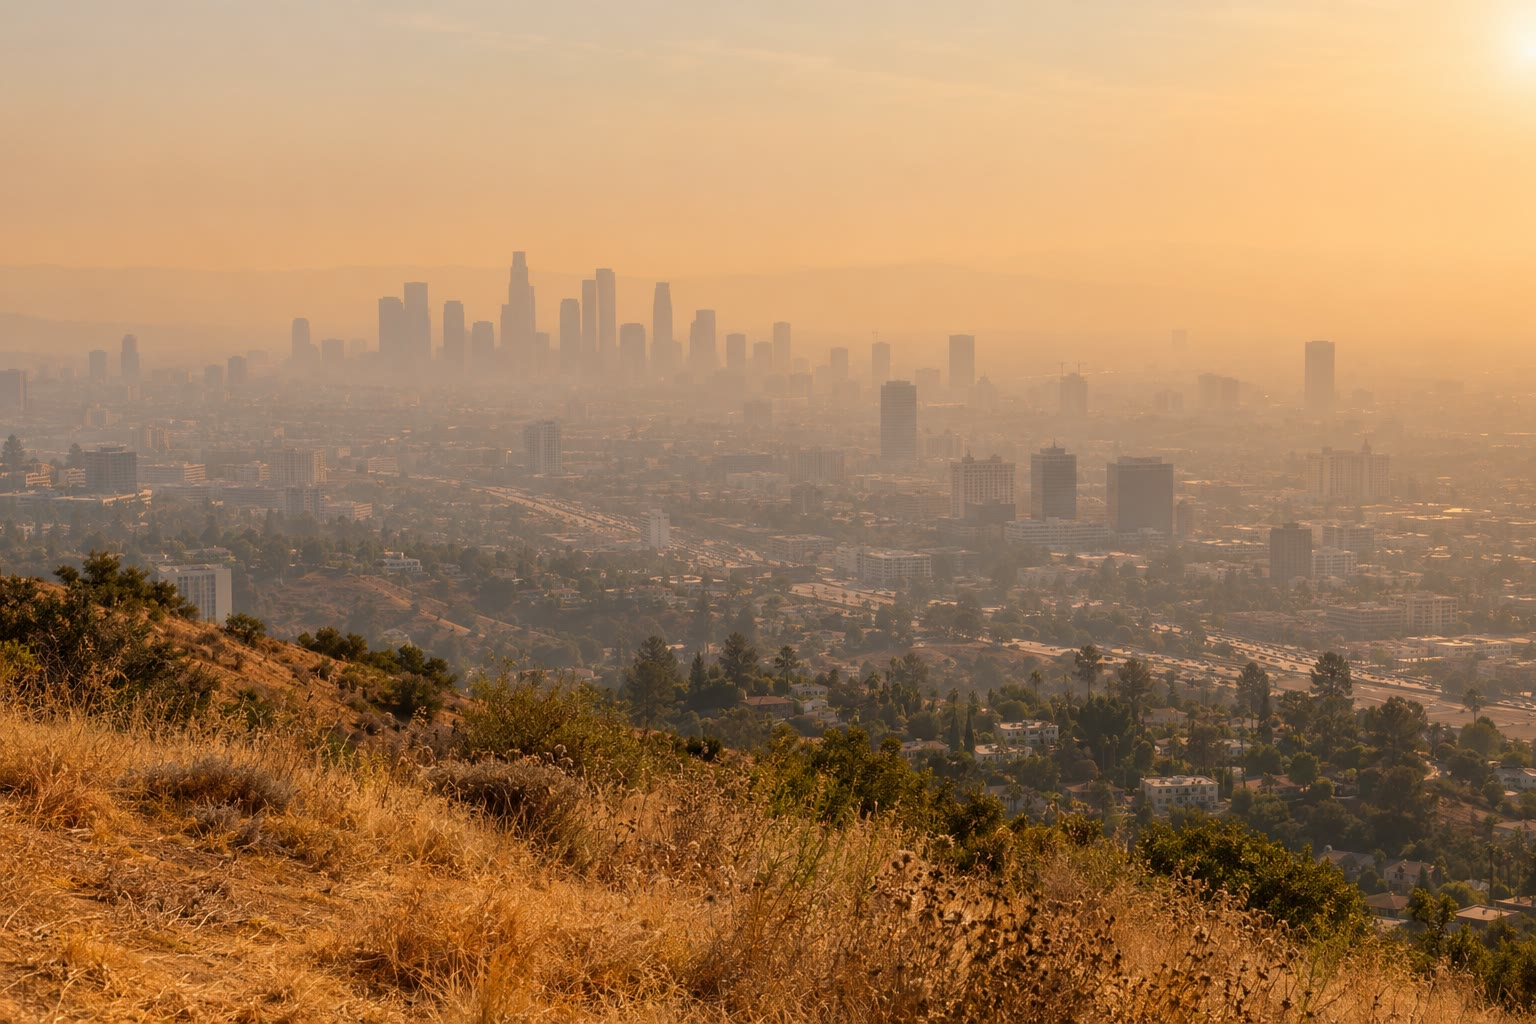
\includegraphics[width=0.6\linewidth]{images/book4/ai/b3-14-smog.jpg}

{\small A city under \omterm{def:b3:photochemistry:smog}{photochemical smog} on a hot afternoon. The brown tint comes
from \ce{NO2}; the ozone, which irritates the lungs, is invisible.}
\end{omfigure}

\begin{omfigure}
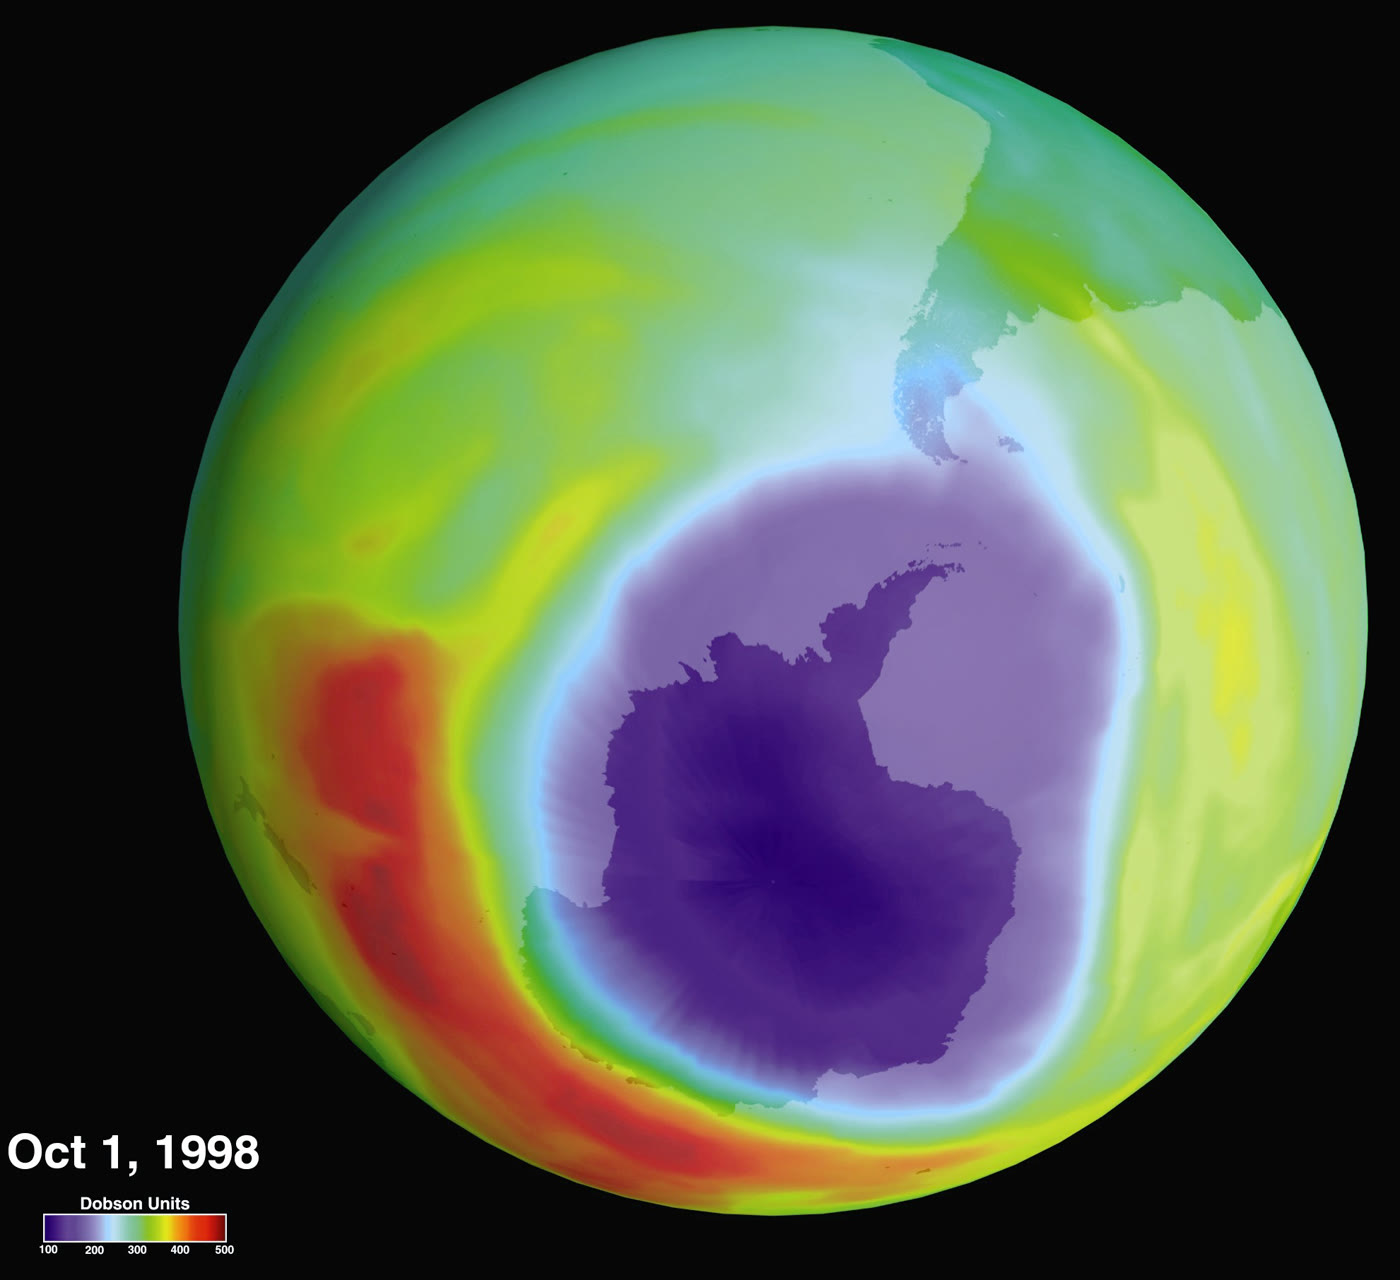
\includegraphics[width=0.5\linewidth]{images/book4/ozone-hole.jpg}

{\small The ozone column over the southern hemisphere on 1 October 1998, from
satellite measurements: the ozone hole over Antarctica (purple) falls to about
100 Dobson units, against about 300 elsewhere.}
\end{omfigure}

\begin{inthelab}[A photoreactor]
A medium-pressure mercury lamp, cooled in a quartz jacket, sits in the centre
of the reaction vessel; a glass filter sleeve removes the wavelengths below
about \qty{300}{nm}, which would destroy the products. The solution is
deoxygenated with a stream of nitrogen (oxygen quenches triplets) and stirred.
The whole reactor is enclosed: the lamp emits ultraviolet light harmful to eyes
and skin, and is never looked at, even briefly.
\end{inthelab}

\begin{safety}{\ghs[0.8cm]{GHS08}\ghs[0.8cm]{GHS09}}
% ledger: ghs4:benzophenone
Benzophenone, a common sensitiser and the reactant of the photoreduction:
suspected of causing cancer, may damage organs after prolonged exposure,
toxic to aquatic life. Weighed and handled with gloves; residues go to the
organic waste.
\end{safety}

\begin{history}[The photochemistry of the future, and the hole in the sky]
In 1912 Giacomo Ciamician, in Bologna, asked whether industry might one day
run on sunlight, as plants do, rather than on coal; he had spent years exposing
flasks of organic compounds to the sun on the roof of his laboratory. In 1985,
three scientists working at an Antarctic research station reported that the
springtime ozone column over it had been falling steeply since the late
1970s.
The ozone hole, explained within a few years by the chemistry of this chapter,
led to the phasing out of chlorofluorocarbons.
\end{history}

\section{Exercises}

\begin{exercise}[$\star$]\label{exo:b3:photochemistry:1}
A lamp delivers \qty{100}{mW} at \qty{365}{nm}. How many photons per second, and how
many einstein per second?
\end{exercise}

\begin{exercise}[$\star$]\label{exo:b3:photochemistry:2}
In \qty{10.0}{min}, a solution absorbing \qty{1.00e-7}{einstein.s^{-1}} converts
\qty{2.0e-5}{mol} of reactant. Compute the \omterm{def:b3:electronic-spectroscopy:quantum-yield}{quantum yield}.
\end{exercise}

\begin{exercise}[$\star$]\label{exo:b3:photochemistry:3}
The photochemical reaction of \ce{H2} with \ce{Cl2} has \omterm{def:b3:electronic-spectroscopy:quantum-yield}{quantum yields} up to $10^4$ and
more. What does this show? Write the propagation steps.
\end{exercise}

\begin{exercise}[$\star$]\label{exo:b3:photochemistry:4}
% ledger: janaf:O.dfH0, janaf:O3.dfH0
From the enthalpies of formation at 0 K of O (\qty{246.79}{kJ/mol}) and \ce{O3}
(\qty{145.35}{kJ/mol}), compute the longest wavelengths that can split \ce{O2} into two
atoms and \ce{O3} into \ce{O2} and O.
\end{exercise}

\begin{exercise}[$\star\star$]\label{exo:b3:photochemistry:5}
A photoswitch has, at \qty{365}{nm}, $\varepsilon_E = 22\,000$ and $\varepsilon_Z = 1500$ \unit{L.mol^{-1}.cm^{-1}}, with
$\Phi_{E\to Z} = 0.11$ and $\Phi_{Z\to E} = 0.40$ (data of the exercise). Compute the photostationary
composition.
\end{exercise}

\begin{exercise}[$\star\star$]\label{exo:b3:photochemistry:6}
Give the products of the \omterm{def:b3:photochemistry:norrish}{Norrish type II reaction} of hexan-2-one, and explain
why pentan-2-one gives ethene rather than propene.
\end{exercise}

\begin{exercise}[$\star\star$]\label{exo:b3:photochemistry:7}
An acceptor has a triplet energy of \qty{250}{kJ/mol}. Among three candidate
sensitisers with triplet energies of 289, 253 and \qty{236}{kJ/mol} (data of the
exercise), which transfers efficiently? Estimate the equilibrium constant of
transfer for each at \qty{298}{K}.
\end{exercise}

\begin{exercise}[$\star\star$]\label{exo:b3:photochemistry:8}
% ledger: kin:O+O2+M.k0, kin:O+O2+M.n
At \qty{230}{K}, with $[\mathrm M] = \qty{4.0e17}{cm^{-3}}$, $[\ce{O2}] = 0.21[\mathrm M]$ and $j_3 = \qty{1.0e-3}{s^{-1}}$,
compute $k_2$ and the steady-state ratio $[\ce{O}]/[\ce{O3}]$.
\end{exercise}

\begin{exercise}[$\star\star$]\label{exo:b3:photochemistry:9}
% ledger: kin:Cl+O3.A, kin:Cl+O3.EaR, kin:Cl+CH4.A, kin:Cl+CH4.EaR
At \qty{230}{K}, compute the rate constants of $\ce{Cl + O3}$ and $\ce{Cl + CH4}$, and the
probability that a Cl atom meets \ce{O3} rather than \ce{CH4} when $[\ce{O3}] = \qty{5.7e12}{cm^{-3}}$
and $[\ce{CH4}] = \qty{4.0e11}{cm^{-3}}$.
\end{exercise}

\begin{exercise}[$\star\star\star$]\label{exo:b3:photochemistry:10}
% ledger: kin:NO+O3.A, kin:NO+O3.EaR
At noon in a city, $[\ce{NO2}]/[\ce{NO}] = 1.5$ and $j_{\ce{NO2}} = \qty{8.0e-3}{s^{-1}}$. Compute the
photostationary ozone at \qty{298}{K} in molecules per \unit{cm^3} and in ppb (air at \qty{1}{bar}).
What happens at night?
\end{exercise}

\begin{exercise}[$\star\star\star$]\label{exo:b3:photochemistry:11}
A \qty{3.0}{mL} solution of absorbance 0.50 at \qty{313}{nm} receives \qty{50}{mW} of
light at that wavelength; the reaction has $\Phi = 0.25$. Compute the initial rate in
\unit{mol.L^{-1}.s^{-1}}.
\end{exercise}

\begin{exercise}[$\star\star\star$]\label{exo:b3:photochemistry:12}
A ferrioxalate actinometer, with a \omterm{def:b3:electronic-spectroscopy:quantum-yield}{quantum yield} of 1.25 at \qty{365}{nm} (data of the
exercise) and total absorption, forms \qty{3.0e-6}{mol} of Fe(II) in \qty{60}{s}.
Compute the \omterm{def:b3:photochemistry:photon-flux}{photon flux}. Why must the conversion stay small?
\end{exercise}

\section{Problem: Making and Unmaking the Ozone Layer}

\begin{problem}[{Weekend problem --- making and unmaking the ozone layer: photon
thresholds, the Chapman steady state with evaluated rate constants, the
chlorine cycle, and the reservoirs that stop it}]
\label{pb:b3:photochemistry:1}
% ledger: janaf:O.dfH0, janaf:O3.dfH0, kin:O+O2+M.k0, kin:O+O2+M.n, kin:O+O3.A, kin:O+O3.EaR, kin:Cl+O3.A, kin:Cl+O3.EaR, kin:O+ClO.A, kin:O+ClO.EaR, kin:Cl+CH4.A, kin:Cl+CH4.EaR, kin:ClO+NO2+M.k0, kin:ClO+NO2+M.n, kin:ClO+NO2+M.kinf, kin:ClO+NO2+M.Fc, oz:column.mean, oz:column.hole
A model of the stratosphere near \qty{30}{km} (data of the problem): $T = \qty{230}{K}$, $[\mathrm M] =
\qty{4.0e17}{cm^{-3}}$, $[\ce{O2}] = 0.21[\mathrm M]$, \omterm{def:b3:photochemistry:photolysis}{photolysis rate constants} $j_1 = \qty{1.0e-11}{s^{-1}}$ (\ce{O2})
and $j_3 = \qty{1.0e-3}{s^{-1}}$ (\ce{O3}), $[\ce{CH4}] = \qty{4.0e11}{cm^{-3}}$, $[\ce{NO2}] = \qty{1.0e9}{cm^{-3}}$. Evaluated rate
constants (\unit{cm^3.s^{-1}}, or \unit{cm^6.s^{-1}} for $k_2$, concentrations being counted per \unit{cm^3}):
$k_2 = \num{6.0e-34}(T/300)^{-2.6}$; $k_4 = \num{8.0e-12}\eu^{-2060/T}$; Cl + \ce{O3}: $\num{2.8e-11}\eu^{-250/T}$;
O + ClO: $\num{2.5e-11}\eu^{110/T}$; Cl + \ce{CH4}: $\num{6.6e-12}\eu^{-1240/T}$; ClO + \ce{NO2} + M: $\num{1.41e-13}$ at
these conditions.

\medskip\noindent\textbf{Part I --- Photon thresholds.}
\begin{enumerate}
  \item Compute $D_0(\ce{O2})$ from $\Delta_fH^\circ_0(\ce{O}) = \qty{246.79}{kJ/mol}$.
  \item Deduce the longest wavelength that splits \ce{O2}.
  \item Compute the energy of $\ce{O3 -> O2 + O}$ ($\Delta_fH^\circ_0(\ce{O3}) = \qty{145.35}{kJ/mol}$) and its
        threshold wavelength.
  \item Visible light could thus split ozone; why is the ultraviolet absorption
        of ozone the one that matters for life?
  \item Why is \ce{O2} photolysed only high in the atmosphere?
\end{enumerate}

\medskip\noindent\textbf{Part II --- The Chapman steady state.}
\begin{enumerate}[resume]
  \item Write the four Chapman steps.
  \item Compute $k_2$ and $k_2[\mathrm M]$ at \qty{230}{K}.
  \item Compute $k_4$.
  \item Compute $[\ce{O}]/[\ce{O3}]$.
  \item Show that $[\ce{O3}] = [\ce{O2}]\sqrt{j_1k_2[\mathrm M]/(j_3k_4)}$.
  \item Compute $[\ce{O3}]$ and its mixing ratio.
  \item Compute $[\ce{O}]$.
  \item Observed ozone is lower than this. Why?
\end{enumerate}

\medskip\noindent\textbf{Part III --- The chlorine cycle.}
\begin{enumerate}[resume]
  \item Write the cycle and its net reaction.
  \item Compute the lifetime of a Cl atom against \ce{O3}.
  \item Compute the lifetime of ClO against O.
  \item Deduce the steady ratio $[\ce{ClO}]/[\ce{Cl}]$.
  \item With $[\ce{Cl}] + [\ce{ClO}] = \qty{1.0e7}{cm^{-3}}$, compare the rate of odd-oxygen loss by the
        cycle with that of the Chapman step $\ce{O + O3}$.
  \item Which step limits the cycle?
\end{enumerate}

\medskip\noindent\textbf{Part IV --- The reservoirs.}
\begin{enumerate}[resume]
  \item Compute the probability that a Cl atom reacts with \ce{O3} rather than with
        \ce{CH4}.
  \item Compute the probability that ClO reacts with O rather than with \ce{NO2}.
  \item Deduce the probability $p$ that a turn of the cycle is completed.
  \item Deduce the mean number of turns before the chlorine is captured.
  \item Explain how polar stratospheric clouds lengthen the chain.
  \item State the result: the number of ozone molecules one chlorine atom
        destroys, in this model, before it is captured in a reservoir.
\end{enumerate}
\end{problem}
